\documentclass[a4paper,12pt]{article}
\usepackage{graphicx}
\usepackage{hyperref}
\usepackage{titlesec}
\usepackage{booktabs}
\usepackage{float}
\usepackage{xcolor}
\usepackage{mathptmx}  % Times New Roman-like font
%\usepackage[backend=biber]{biblatex}



\title{\textbf{Speech Understanding}\\
\bigskip
\bigskip
\bigskip
{Programming Assignment-1}\\
\bigskip\bigskip\bigskip
{Project Report - Q-2-Task B} 
\bigskip\bigskip\bigskip\\
    {Comparative Analysis of \\Spectrograms Across Music Genres}
}
\bigskip\bigskip\bigskip

\author{\textbf{Prepared By:}\\Om Prakash Solanki (M23CSA521)}

\begin{document}
\maketitle

\newpage
\tableofcontents
\newpage

\newpage
\section{Objective}
The objective of Task is to analyze and compare the sound characteristics of four different music genres—Pop, HipHop, Classical, and Jazz—by generating and examining their spectrograms. Spectrograms are visual representations of sound that show how frequencies change over time. By selecting one song from each genre, creating their spectrograms, and comparing them, we can observe how each genre uses frequency ranges, energy distribution, and temporal patterns differently. 
\newpage
\section{List of Songs Selected for Analysis}
For this task, four songs from four different genres were selected to ensure a diverse and comprehensive analysis. The songs chosen are:
\subsection{Pop Genre: "Alive" by Songwriterz}
This song represents the Pop genre, known for its catchy melodies, strong vocals, and consistent rhythms. The spectrogram is expected to show clear vocal patterns and a prominent bassline.
\subsection{HipHop Genre: "Into You" by Tom Orlando}
This track represents the HipHop genre, characterized by strong beats, rhythmic patterns, and deep basslines. The spectrogram will likely highlight the dominant low-frequency beats and rhythmic vocal delivery.
\subsection{Classical Genre: "Shauna's Theme" by Jorgen Kruse}
This piece represents the Classical genre, known for its balanced frequency range, smooth transitions, and melodic instrumentation. The spectrogram is expected to show a wide and even distribution of frequencies, reflecting the use of orchestral instruments.
\subsection{Jazz Genre: "Athens" by Pierce Murphy}
This song represents the Jazz genre, which is known for its improvisational nature, wide frequency range, and dynamic energy. The spectrogram will likely display varied patterns and a mix of low, mid, and high frequencies, reflecting the use of instruments like the saxophone, piano, and double bass.
\newpage
\section{Spectrogram Analysis}
\subsection{Song 1: Analysis of the Spectrogram for Pop Genre}
\begin{figure}[H]
    \centering
    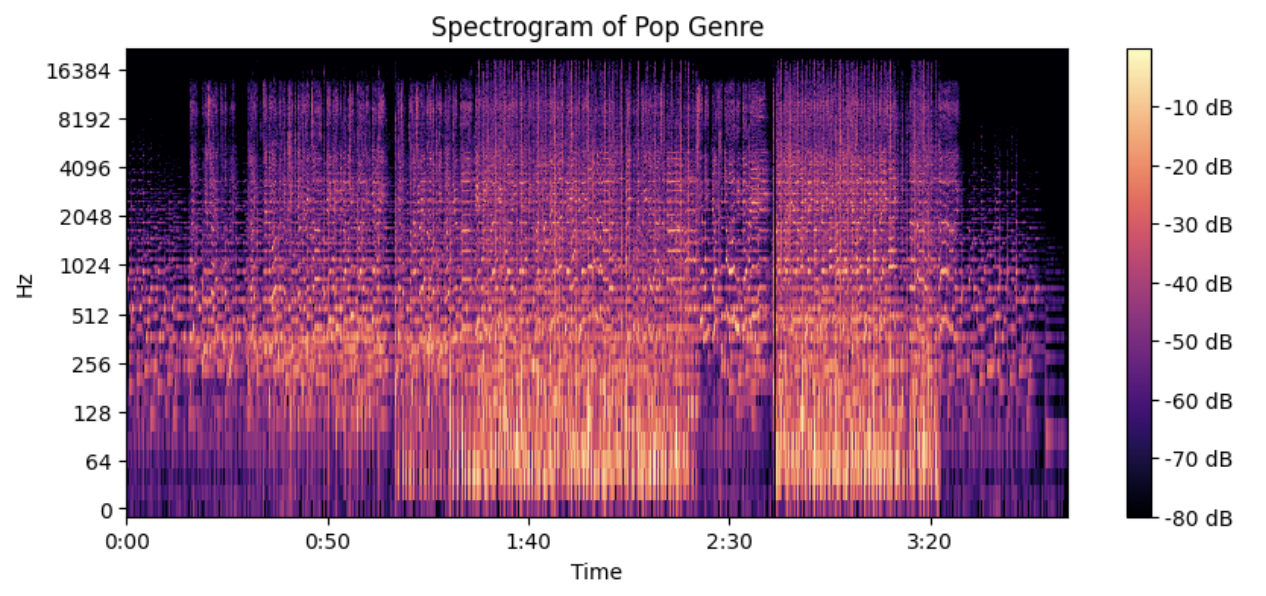
\includegraphics[width=1\linewidth]{1.png}
    \caption{Spectrogram of Pop Genre}
\end{figure}
The spectrogram provided for the Pop genre can be analyzed based on the following characteristics:
\subsubsection{Frequency Range:}
\begin{itemize}
    \item The spectrogram shows a wide frequency range, which is typical for Pop music.
    \item \textbf{Low Frequencies (Bottom of the Spectrogram):} Strong bass presence, indicating the use of bass instruments or electronic bass lines.
\item \textbf{Mid Frequencies (256 - 4096 Hz):} Clear and consistent patterns, likely representing vocals, guitars and melodic instruments. This is where most pop music sounds are concentrated.
\item \textbf{High Frequencies (Top of the Spectrogram):} Less energy compared to low and mid frequencies, but still present, possibly due to high-pitched instruments.
\end{itemize}
\subsubsection{Temporal Patterns:}
\begin{itemize}
    \item The spectrogram shows repetitive patterns over time, which is characteristic of Pop music's structured and predictable rhythm.
    \item \textbf{0:00 - 0:50:} The beginning of the song likely has a consistent beat and melody, with clear vocal lines.
    \item \textbf{0:50 - 1:40:} The intensity may increase, possibly indicating a more energetic section.
    \item \textbf{1:40 - 2:30:} The patterns remain consistent, suggesting a return to the verse or a bridge section.
    \item \textbf{2:30 - 3:20:} The end of the song may show a gradual decrease in intensity, possibly fading out or transitioning to a softer section.
\end{itemize}
\subsubsection{Spectral Density:}
\begin{itemize}
    \item The energy distribution is concentrated in the low and mid frequencies, which is typical for Pop music.
    \item \textbf{Low Frequencies:} High energy, indicating a strong bassline.
    \item \textbf{Mid Frequencies:} Moderate to high energy, representing vocals and melodic instruments.
    \item \textbf{High Frequencies:} Lower energy, but still present, possibly due to cymbals or high-pitched synths.
\end{itemize}
\subsubsection{Dynamic Range:}
\begin{itemize}
    \item The dynamic range (difference between the quietest and loudest parts) is moderate, which is typical for Pop music.
    \item The spectrogram shows consistent energy levels, with occasional peaks (e.g., during the chorus or instrumental breaks).
\end{itemize}
\subsubsection{Time-Domain Characteristics:}
\begin{itemize}
    \item The spectrogram shows smooth transitions between sections, indicating a well-structured song.
    \item There are no abrupt changes in intensity, which is typical for Pop music's polished production.
\end{itemize}
\subsubsection{Key Observations:}

\begin{enumerate}
    \item Strong Bass Presence:
        \begin{itemize}
            \item The low frequencies (bottom of the spectrogram) show high energy, indicating a prominent bassline, which is common in Pop music.    
        \end{itemize}
    \item Clear Vocals:
        \begin{itemize}
            \item The mid frequencies show consistent patterns, likely representing vocals. This is a hallmark of Pop music, where vocals are often the focal point.   
        \end{itemize}
    \item Repetitive Patterns:
        \begin{itemize}
            \item The spectrogram shows repetitive patterns over time, indicating a structured and predictable rhythm, typical of Pop music.   
        \end{itemize}
    \item Moderate Dynamic Range:
        \begin{itemize}
            \item The energy levels are consistent, with occasional peaks, suggesting a balanced mix with no extreme variations in volume.  
        \end{itemize}
\end{enumerate}
\newpage
\subsection{Song 2: Analysis of the Spectrogram for HipHop Genre}
\begin{figure}[H]
    \centering
    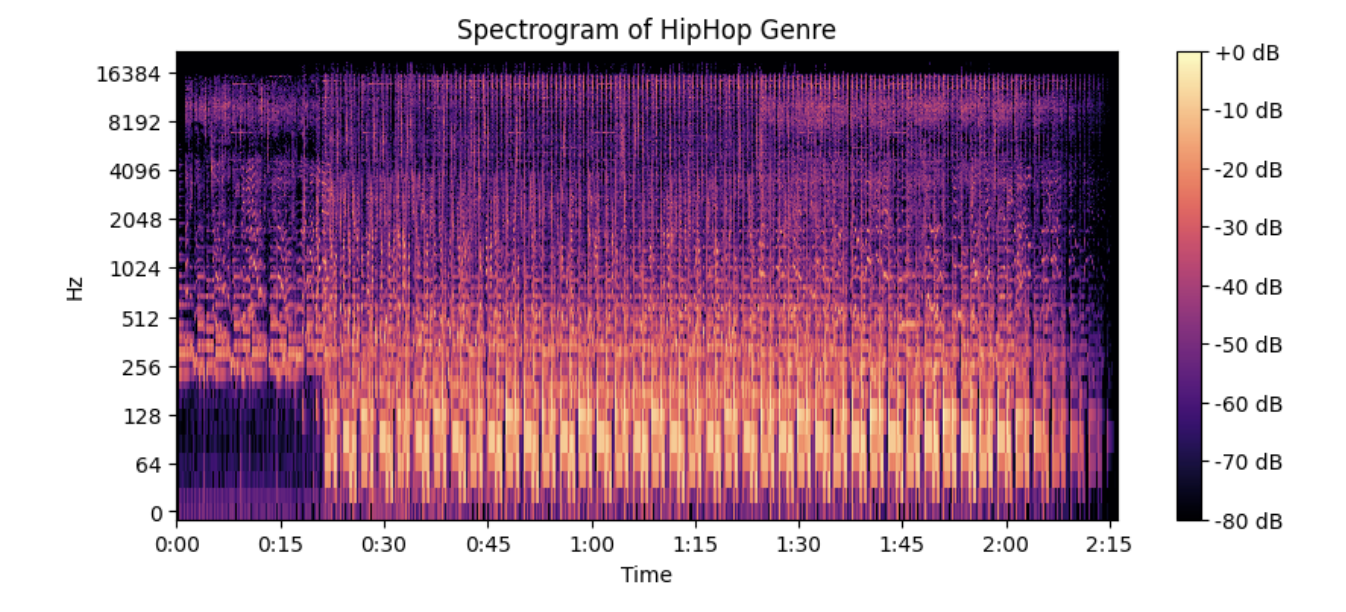
\includegraphics[width=1\linewidth]{2.png}
    \caption{Spectrogram of Hip Hop Genre}
\end{figure}
The spectrogram provided for the HipHop genre can be analyzed in simple terms based on the following characteristics:

\subsubsection{Frequency Range:}
\begin{itemize}
    \item \textbf{Low Frequencies (Bottom of the Spectrogram):} Strong and consistent bass presence, which is typical for HipHop music. This represents the deep basslines and beats that are a key part of the genre.
    \item \textbf{Mid Frequencies:} Less energy compared to the bass, but still present. This could be due to vocals or rhythmic elements like snares and hi-hats.
    \item \textbf{High Frequencies (Top of the Spectrogram):} Minimal energy, which is common in HipHop as the focus is more on bass and rhythm rather than high-pitched sounds.
\end{itemize}
\subsubsection{Temporal Patterns:}
\begin{itemize}
    \item The spectrogram shows strong, repetitive patterns over time, which is characteristic of HipHop's rhythmic and beat-driven nature.
    \item \textbf{0:00 - 0:30:} The beginning of the song likely has a strong beat and bassline, setting the rhythm.
    \item \textbf{0:30 - 1:00:} The intensity remains consistent, possibly with added vocal elements or instrumental layers.
    \item \textbf{1:00 - 1:30:} The patterns continue to repeat, indicating a steady rhythm typical of HipHop.
    \item \textbf{1:30 - 2:00:} The end of the song may show slight variations, but the overall rhythm remains strong and consistent.
\end{itemize}
\subsubsection{Spectral Density:}
\begin{itemize}
    \item The energy distribution is heavily concentrated in the low frequencies, which is typical for HipHop music.
    \item \textbf{Low Frequencies:} High energy, indicating a strong bassline and beats.
    \item \textbf{Mid Frequencies:} Moderate energy, representing vocals or rhythmic elements like snares.
    \item \textbf{High Frequencies:} Very low energy, as HipHop typically doesn’t focus on high-pitched sounds.
\end{itemize}
\subsubsection{Dynamic Range:}
\begin{itemize}
    \item The dynamic range (difference between the quietest and loudest parts) is relatively narrow, which is common in HipHop. The beats and bass are consistently strong throughout the song.
\end{itemize}
\subsubsection{Time-Domain Characteristics:}
\begin{itemize}
    \item The spectrogram shows consistent energy levels over time, with no abrupt changes. This reflects the steady and rhythmic nature of HipHop music.
\end{itemize}
\subsubsection{Key Observations:}

\begin{enumerate}
    \item Strong Bass and Beats:
        \begin{itemize}
            \item The low frequencies (bottom of the spectrogram) show high energy, indicating a strong bassline and beats, which are central to HipHop music.  
        \end{itemize}
    \item Repetitive Rhythms:
        \begin{itemize}
            \item The spectrogram shows repetitive patterns over time, reflecting the steady and rhythmic nature of HipHop. 
        \end{itemize}
    \item Minimal High Frequencies:
        \begin{itemize}
            \item The high frequencies (top of the spectrogram) have very low energy, as HipHop music typically doesn’t focus on high-pitched sounds.   
        \end{itemize}
    \item Consistent Energy:
        \begin{itemize}
            \item The energy levels are consistent throughout the song, with no major peaks or drops, indicating a steady and rhythmic track.  
        \end{itemize}
\end{enumerate}
\newpage
\subsection{Song 3: Analysis of the Spectrogram for Jazz Genre}
\begin{figure}[H]
    \centering
    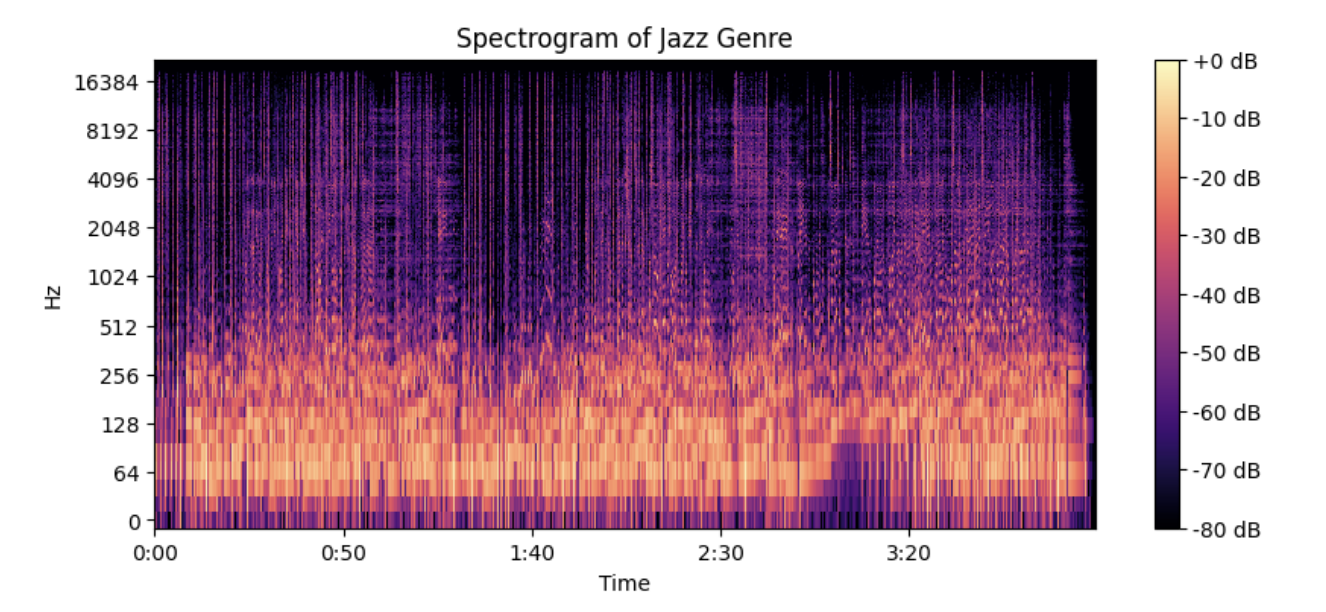
\includegraphics[width=1\linewidth]{4.png}
    \caption{Spectrogram of Jazz Genre}
\end{figure}
The spectrogram provided for the Jazz genre can be analyzed in simple terms based on the following characteristics:
\subsubsection{Frequency Range:}
\begin{itemize}
    \item \textbf{Low Frequencies (Bottom of the Spectrogram):} Moderate energy, representing instruments like the double bass or bass guitar, which are common in Jazz.
    \item \textbf{Mid Frequencies:} High energy, likely due to instruments like the piano, saxophone, or trumpet, which are central to Jazz music.
    \item \textbf{High Frequencies (Top of the Spectrogram):} Moderate to high energy, possibly from cymbals, high-pitched saxophone notes, or other melodic instruments.
\end{itemize}
\subsubsection{Temporal Patterns:}
\begin{itemize}
    \item The spectrogram shows varied and dynamic patterns over time, which is typical for Jazz due to its improvisational nature.
    \item \textbf{0:00 - 0:50:} The beginning of the song may have a smooth and flowing rhythm, with instruments like the piano or saxophone taking the lead.
    \item \textbf{0:50 - 1:40:} The intensity may increase, possibly indicating a solo section or a more energetic part of the song.
    \item \textbf{1:40 - 2:30:} The patterns may change, reflecting the improvisational nature of Jazz, with different instruments taking turns to shine.
    \item \textbf{2:30 - 3:20:} The end of the song may show a gradual decrease in intensity, possibly fading out or transitioning to a softer section.
\end{itemize}
\subsubsection{Spectral Density:}
\begin{itemize}
    \item The energy distribution is balanced across low, mid, and high frequencies, which is typical for Jazz music.
    \item \textbf{Low Frequencies:} Moderate energy, representing bass instruments.
    \item \textbf{Mid Frequencies:} High energy, representing melodic instruments like the piano, saxophone, or trumpet.
    \item \textbf{High Frequencies:} Moderate to high energy, possibly from cymbals or high-pitched notes.
\end{itemize}
\subsubsection{Dynamic Range:}
\begin{itemize}
    \item The dynamic range (difference between the quietest and loudest parts) is wide, which is common in Jazz. This reflects the genre's expressive and dynamic nature.
\end{itemize}
\subsubsection{Time-Domain Characteristics:}
\begin{itemize}
    \item The spectrogram shows smooth and flowing transitions between sections, indicating the improvisational and expressive nature of Jazz music.
\end{itemize}
\subsubsection{Key Observations:}

\begin{enumerate}
    \item Balanced Frequency Range:
        \begin{itemize}
            \item The spectrogram shows energy across low, mid, and high frequencies, reflecting the diverse range of instruments used in Jazz.  
        \end{itemize}
    \item Dynamic and Varied Patterns:
        \begin{itemize}
            \item The spectrogram shows varied patterns over time, reflecting the improvisational and expressive nature of Jazz. 
        \end{itemize}
    \item Wide Dynamic Range:
        \begin{itemize}
            \item The energy levels vary significantly, indicating the expressive and dynamic nature of Jazz music.   
        \end{itemize}
    \item Smooth Transitions:
        \begin{itemize}
            \item The transitions between sections are smooth and flowing, typical of Jazz's improvisational style.
        \end{itemize}
\end{enumerate}
\newpage
\subsection{Song 4: Analysis of the Spectrogram for Classical Genre}
\begin{figure}[H]
    \centering
    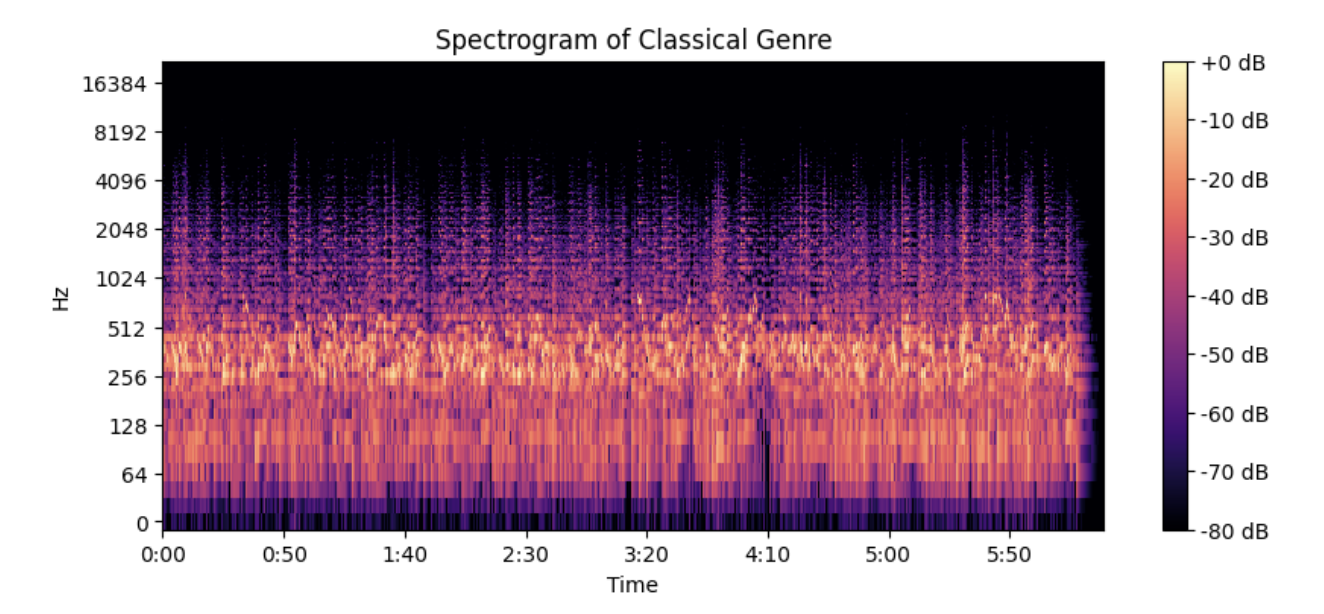
\includegraphics[width=1\linewidth]{3.png}
    \caption{Spectrogram of Classical Genre}
\end{figure}
The spectrogram provided for the Classical genre can be analyzed based on the following characteristics:
\subsubsection{Frequency Range:}
\begin{itemize}
    \item \textbf{Low Frequencies (Bottom of the Spectrogram):}
    \begin{itemize}
        \item Strong presence, representing bass instruments such as cellos and double bass.
        \item Classical music often contains rich low-frequency components that provide a warm and deep foundation.
        \end{itemize}
    \item \textbf{Mid Frequencies:} 
        \begin{itemize}
        \item Moderate to high energy, primarily from string instruments (violins, violas), pianos, and woodwinds (flutes, clarinets).
        \item These frequencies define the melody and harmony, which are central to classical compositions.
        \end{itemize}
    \item \textbf{High Frequencies (Top of the Spectrogram):}
        \begin{itemize}
        \item Less dense but still present, representing higher-pitched instruments like the piccolo, high violin notes, or cymbals.
        \item The energy is not as intense as in rock or jazz but remains steady and smooth.
        \end{itemize}
\end{itemize}
\subsubsection{Temporal Patterns:}
\begin{itemize}
    \item The spectrogram shows a gradual and structured evolution over time, which is typical of classical compositions.
    \item Classical music often follows a smooth and flowing structure without sudden bursts of high-energy transients.
    \item \textbf{0:00 - 1:40:} The beginning of the piece shows steady, moderate energy, possibly representing a slow introduction.
    \item \textbf{1:40 - 3:20:} The intensity slightly increases, which could indicate a section with more instrumental layering.
    \item \textbf{3:20 - 5:00:} Variations in intensity appear, possibly representing dynamic contrasts (crescendo or decrescendo).
    \item \textbf{5:00 - End:} The spectrogram shows a gradual decrease in intensity, possibly leading to a soft ending.
\end{itemize}
\subsubsection{Spectral Density:}
\begin{itemize}
    \item \textbf{Low Frequencies:}  Strong and consistent, representing deep orchestral instruments.
    \item \textbf{Mid Frequencies:} Well-balanced, reflecting the harmonics and interplay between different instruments.
    \item \textbf{High Frequencies:} Present but not overly dominant, indicating a focus on harmony and melody rather than percussive or transient-heavy elements.
\end{itemize}
\subsubsection{Dynamic Range:}
\begin{itemize}
    \item Classical music typically has a wide dynamic range, with moments of very soft and very loud passages.
    \item The spectrogram reflects this, showing areas of varying intensity, indicating dynamic expression within the composition.
\end{itemize}
\subsubsection{Time-Domain Characteristics:}
\begin{itemize}
    \item Smooth and flowing transitions between sections.
    \item No abrupt peaks or sudden changes, which is expected in classical music.
    \item The lack of sharp, transient energy suggests a continuous and harmonically rich sound, unlike electronic or percussive-heavy genres.

\end{itemize}
\subsubsection{Key Observations:}

\begin{enumerate}
    \item Balanced Frequency Range:
        \begin{itemize}
            \item The spectrogram shows energy across low, mid, and high frequencies, reflecting the diverse instrumentation in classical music.  
        \end{itemize}
    \item Smooth and Gradual Transitions:
        \begin{itemize}
            \item The spectrogram does not show sudden jumps in intensity, aligning with the flowing nature of classical compositions.
        \end{itemize}
    \item Wide Dynamic Range:
        \begin{itemize}
            \item There are visible variations in intensity, indicating expressive dynamics, a key feature of classical music.  
        \end{itemize}
    \item Minimal Transient Energy:
        \begin{itemize}
            \item Unlike jazz, rock, or pop, there are no sharp bursts of energy, confirming that the composition is more harmonically structured than rhythmically driven.
        \end{itemize}
\end{enumerate}

\newpage
\section{Comparative Analysis of Spectrograms of Four Genres}
\subsection{Pop Genre}
\begin{itemize}
    \item \textbf{Frequency Range:} Strong bass (low frequencies) and clear mid-frequencies (vocals and melodic instruments). High frequencies are present but less dominant.
    \item \textbf{Temporal Patterns:} Repetitive and structured rhythms, with consistent energy and occasional peaks during choruses.
    \item \textbf{Key Observations:} Strong basslines, clear vocals, and predictable rhythms make Pop music catchy and easy to follow.
\end{itemize}

\subsection{HipHop Genre}
\begin{itemize}
    \item \textbf{Frequency Range:} Very strong bass (low frequencies) and moderate mid-frequencies (vocals and beats). High frequencies are minimal.
    \item \textbf{Temporal Patterns:} Strong, repetitive beats with steady energy throughout the song.
    \item \textbf{Key Observations:} Dominant basslines and rhythmic beats are the focus, with minimal high-frequency energy.
\end{itemize}


\subsection{Jazz Genre}
\begin{itemize}
    \item \textbf{Frequency Range:} Balanced across low, mid, and high frequencies, with moderate bass, strong mid-frequencies (saxophone, piano), and moderate highs (cymbals).
    \item \textbf{Temporal Patterns:} Varied and dynamic patterns, reflecting improvisation and expressive solos.
    \item \textbf{Key Observations:} Wide dynamic range and smooth transitions highlight Jazz’s improvisational and diverse instrumentation.
\end{itemize}


\subsection{Classical Genre}
\begin{itemize}
    \item \textbf{Frequency Range:} Balanced across low (cellos, bass), mid (violins, piano), and high frequencies (piccolo, cymbals), with smooth energy distribution.
    \item \textbf{Temporal Patterns:} Gradual and structured evolution, with smooth transitions and no abrupt changes.
    \item \textbf{Key Observations:} Wide dynamic range and harmonic richness, with a focus on melody and harmony rather than rhythm.
\end{itemize}
\newpage
\section{Summary}
\begin{itemize}
    \item \textbf{Pop:} Strong bass and vocals, repetitive rhythms, and moderate dynamics.
    \item   \textbf{HipHop:} Dominant bass and beats, steady rhythms, and minimal highs.
    \item \textbf{Jazz:} Balanced frequencies, dynamic patterns, and improvisational style.
    \item \textbf{Classical:} Smooth transitions, wide dynamics, and harmonic richness.
\end{itemize}
Each genre has unique characteristics that are clearly reflected in their spectrograms, making them distinct in terms of frequency range, rhythm, and energy distribution.


\newpage
\section{Code Repository} 
\href{https://github.com/IITJ-M23CSA521/M23CSA521_PA1.git}{GitHub Repository URL}

\addcontentsline{toc}{section}{References}
%\addbibresource{references.bib}
%\printbibliography[heading=bibintoc, title={References}]
\begin{thebibliography}{9}
    \bibitem{example} \href{https://www.kaggle.com/code/sujaykapadnis/audio-machine-learning-for-speech-recog-intro}{Audio Machine Learning for speech Recog Intro}
    \bibitem{example2} \href{https://www.kaggle.com/code/jerrypeng/dsp-tutorial-3-demos-for-speech-processing}{DSP Tutorial 3: Demos for speech processing}
    \bibitem{example3} \href{https://www.kaggle.com/code/santoshkumar/understanding-audio-data-getting-started}{Understanding-audio-data[getting-started]}
    \bibitem{Songs} \href{https://www.jamendo.com/start}{Songs Website}
\end{thebibliography}

\end{document}
